
\subsubsection{AC-3}
\lezione{Lezione 11}{4/11/2024}
Un famoso algoritmo che risolve CSP sfruttando le arc-consistencies è l'\textbf{AC-3}:
\medskip
\tikzstyle{startstop} = [rectangle, rounded corners, minimum width=3cm, minimum height=1cm,text centered, draw=black, fill=red!30]
\tikzstyle{process} = [rectangle, minimum width=3cm, minimum height=1cm, text centered, draw=black, fill=blue!30]
\tikzstyle{decision} = [diamond, minimum width=3cm, minimum height=1cm, text centered, draw=black, fill=green!30]
\tikzstyle{arrow} = [thick,->,>=stealth]
\tikzstyle{io} = [trapezium, trapezium left angle=70, trapezium right angle=110, minimum width=3cm, minimum height=1cm, text centered, draw=black, fill=orange!30]


\begin{tikzpicture}[node distance=2cm]

% Nodes
\node (start) [startstop] {Inizio};
\node (initialize) [process, below of=start] {Inizializza coda con tutti gli archi del grafo};
\node (checkqueue) [decision, below of=initialize, yshift=-0.5cm] {Coda vuota?};
\node (dequeue) [process, right of=checkqueue, xshift=5cm] {Estrai un arco (Xi, Xj) dalla coda};
\node (revise) [process, below of=dequeue] {Aggiorna (Xi, Xj)};
\node (revised) [decision, below of=revise, yshift=-1cm] {Aggiornato?};
\node (addneighbors) [process, left of=revised, xshift=-5cm] {Aggiungi alla coda tutti gli archi (Xk, Xi)};
\node (end) [startstop, below of=checkqueue, yshift=-1cm] {Fine};

% Arrows
\draw [arrow] (start) -- (initialize);
\draw [arrow] (initialize) -- (checkqueue);
\draw [arrow] (checkqueue.east) -- ++(1,0) node[midway,above] {No} |- (dequeue.west) ;
\draw [arrow] (dequeue) -- (revise);
\draw [arrow] (revise) -- (revised);
\draw [arrow] (revised.west) -- ++(-1,0) |- (addneighbors.east);
\draw [arrow] (addneighbors.west) -- ++(-0.5,0) -- ++(0,5) |- (checkqueue.west);
\draw [arrow] (checkqueue.south) -- ++(0,-0.5) node[midway,right] {Sì} -| (end.north);
%\draw [arrow] (revised.south) -- ++(0,-0.5) node[midway,right] {No} |- (checkqueue.north);

\end{tikzpicture}

\subsubsection{Path Consistency}
Possiamo considerare la \textbf{Node Consistency} come consistenza di \textbf{ordine 0} e la \textbf{Arc Consistency} una
consistenza di \textbf{ordine 1}. Con questo ragionamento possiamo estendere il concetto di consistenza a \textbf{ordine 3}, 
anche detta \textbf{path-consistency} e ad un generico \textbf{ordine n}.\\
\paragraph{Definizione.}Per ogni assegnamento $(A,B)$ legale (ossia arc-consistent), $C$ è  path consistent con $(A,B)$ sse
$\exists v \in C$ tale che:
\begin{equation}
    \begin{cases}
        C \text{ arc-consistent con } A\\
        C \text{ arc-consistent con } B 
    \end{cases}
\end{equation}

\subsubsection{Backtracking Search}
Un altro algoritmo usato per la risoluzione dei CSP è il Backtracking Search: dato un vettore di $n$ variabili
$\Gamma = \left\langle x_1, x_2, \dots, x_n\right\rangle $, ad ogni step si prova ad assegnare un valore ad una variabile.
In particolare:
\begin{enumerate}
    \item \textbf{Start}: si parte con l'assegnamento nullo $\Gamma = \emptyset$
    \item \textbf{Espansione del Nodo}: fintanto che non ho trovato un assegnamento valido, scelgo un valore per una variabile
    \item \textbf{Backtracking}: se mi accorgo che l'assegnamento mi porta ad un vicolo cieco, ritorno indietro e provo con un nuovo assegnamento.
\end{enumerate}
Chiaramente l'algoritmo affronta un approccio esaustivo e, nel caso peggiore, il numero di assegnamenti da provare è $m^n$ dove
$m$ è la dimensione del dominio e $n$ è il numero di variabili. A differenza dei problemi di search, tuttavia, in questo caso
non siamo interessati all'ordine degli assegnamenti ed è per questo motivo che possiamo scegliere arbitrariamente un ordine sia per i valori
che per le variabili senza invalidare l'ammissibilità di $\Gamma$ 
\subsubsection{Ordering Delle Variabili}
Per ottimizzare il backtracking, possiamo implementare delle euristiche che scelgono il prossimo nodo da espandere:
\paragraph{Ordine Lessicografico}è un ordine statico, unfair e quasi mai utile.
\paragraph{Ordine Random}è dinamico e a differenza del precedente è più fair
\paragraph{Euristica di Grado (EG)}con questa euristica si sceglie sempre prima la variabile con il \textbf{maggior numero di vincoli} che 
vincolano variabili ancora non assegnate
\paragraph{Minimum Remain Value (MRV)}Si scelgono le variabili con i domini più piccoli

I classici solutori CSP basati su backtracking di solito sono basati su \textbf{EG} e in caso di spareggio vengono usati \textbf{EG + MRV}.
Il grande vantaggio di usare EG o MRV è il fatto che conducono subito a \textbf{vicoli ciechi}, cioè sollecitano il principio di
\textbf{fail-first} in modo da escludere a monte molti percorsi fallimentari e non accorgersene troppo tardi.
\subsubsection{Euristica per i Valori}
Anche per i valori da assegnare è possibile realizzare delle euristiche apposite, come il \textbf{Least Constraining Value (LCV)}:
questa euristica sceglie i valori che escludono \textbf{meno valori possibili} nei domini delle altre variabili.

Implementare \textbf{EG/MRV} e \textbf{LCV}, che hanno tendenze opposte, funzionano bene insieme: se le prime 2 euristiche ci avvicinano ai vicoli ciechi
la LCV ci allontana scegliendo i valori che soddisfano più vincoli possibili. In questa maniera si evitano a tutti i costi i backtracking.

\paragraph{Forward Checking}
Questa tecnica, basata sulla \textbf{constraint propagation}, consiste nell'escludere apriori tutti i nodi che, se espansi, so già
che portino a vicoli ciechi.

\subsection{Local Search}
Nel mondo del CSP possiamo dire che esistano 2 scuole di pensiero: la prima scuola è quella \textit{costruttiva}, cioè a partire da un assegnamento
vuoto ci costruiamo man mano lo stato ammissibile. Un altra scuola di pensiero ragiona al contrario: a partire da un assegnamento con valori random inammissibile
lo si aggiusta man mano fino ad avere uno stato ammissibile; questo approccio è detto \textbf{ricerca locale}.
\subsubsection{Min Conflicts}
Quest'algoritmo è basato su ricerca locale: 
\begin{enumerate}
    \item \textbf{Start}: si parte inizialmente con uno stato le cui variabili hanno assegnamenti tutti casuali.
    \item \textbf{Step}: fintanto che non si è raggiunto uno stato ammissible, si trasforma l'assegnamento $\Gamma_1$ in $\Gamma_2$
    tale che viola un numero di vincoli minore rispetto all'assegnamento precedente (ossia cerchiamo la soluzione che è \textbf{localmente migliore}).
\end{enumerate}
Teoricamente quest'algoritmo è pessimo:
\begin{itemize}
    \item Non è un algoritmo \textbf{Anytime}
    \item Non garantisce di trovare una soluzione ottima \textbf{tempo finito (anche esponenziale)}.
\end{itemize}
Eppure, empiricamente, è \textbf{molto efficiente}: riesce a risolvere il problema delle n regine in \textbf{qualche decina di iterazioni}.
Possiamo dire in generale che:
\begin{itemize}
    \item \textbf{Minconflicts} funziona bene nelle istanze di problema con \textbf{molte variabili e pochi vincoli}
    \item \textbf{Backtracking Search} funziona bene nelle istanze di problema con \textbf{molti vincoli e poche variabili}
\end{itemize}
Questo perchè, a differenza di molte altre classi di problemi, i problemi CSP sono fortemente influenzati non direttamente dal
numero di variabili o di valori ma dal loro rapporto. Esiste infatti un grafico che riesce a mettere in relazione la difficoltà
di un problema di CSP con il rapporto di variabili/vincoli, ed emerge che esiste un punto critico in cui la difficolta cresce vertiginosamente.

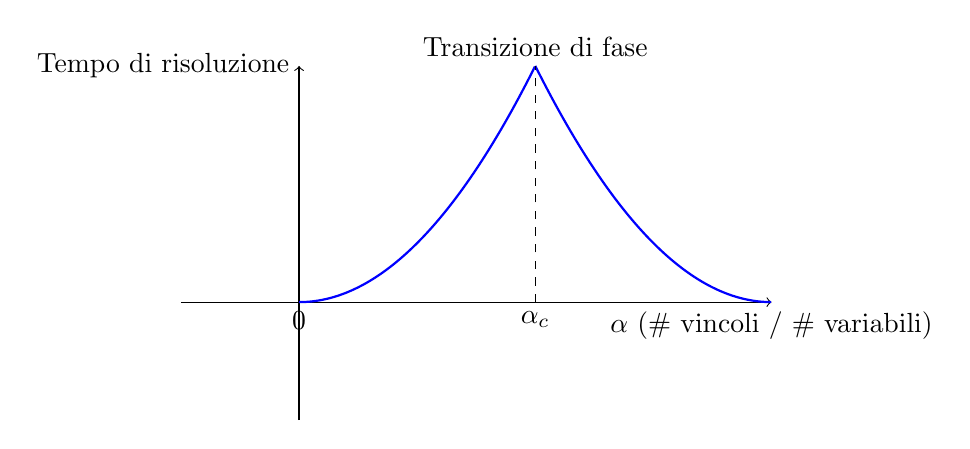
\begin{tikzpicture}[scale=3]

    % Assi
    \draw[->] (-0.5,0) -- (2,0) node[below] {$\alpha$ (\# vincoli / \# variabili)};
    \draw[->] (0,-0.5) -- (0,1) node[left] {Tempo di risoluzione};
    
    % Curva precisa
    \draw[thick,blue,smooth,domain=0:1,samples=100] 
        plot (\x,{(\x)^2}); % Parte sottovincolata
    \draw[thick,blue,smooth,domain=1:2,samples=100] 
        plot (\x,{(2 - \x)^2}); % Parte sovra-vincolata
    
    % Aggiunta annotazioni
    \draw[dashed] (1,0) -- (1,1) node[above] {Transizione di fase};
    
    % Etichette
    \node[below] at (1,0) {$\alpha_c$};
    \node[below] at (0,0) {0};
    
    \end{tikzpicture}